% The Alembic — workflow as a distillation column.
% Compile: pdflatex alembic_workflow  (standalone → cropped vector PDF)
\documentclass[border=6pt]{standalone}
\usepackage[T1]{fontenc}
\usepackage{ebgaramond}
\usepackage{amssymb}
\usepackage{xcolor}
\usepackage{tikz}
\usetikzlibrary{positioning,shapes.geometric,arrows.meta,backgrounds,calc,fit,
                decorations.pathmorphing,shadows.blur}

% ---- alchemic palette (parchment, sepia ink, gold, verdigris, ember) ----
\definecolor{parch}{RGB}{246,240,226}
\definecolor{parchD}{RGB}{238,229,208}
\definecolor{ink}{RGB}{68,52,38}
\definecolor{gold}{RGB}{176,136,56}
\definecolor{verd}{RGB}{68,110,101}
\definecolor{ember}{RGB}{150,72,40}

\tikzset{
  vessel/.style={draw=ink, line width=0.9pt, rounded corners=7pt,
    minimum width=5.3cm, minimum height=1.2cm, align=center, text=ink,
    blur shadow={shadow xshift=1.1pt, shadow yshift=-1.3pt, shadow opacity=28}},
  neck/.style={draw=ink, line width=0.9pt, fill=parchD},
  seal/.style={draw=verd!72!black, line width=1.1pt, fill=verd, circle,
    minimum size=0.92cm, inner sep=0pt, text=parch, font=\bfseries\small,
    blur shadow={shadow xshift=0.8pt, shadow yshift=-0.9pt, shadow opacity=26}},
  endcap/.style={draw=ink, line width=1pt, align=center, text=ink},
  descbox/.style={anchor=west, align=left, text width=8.9cm, font=\small, text=ink},
  flow/.style={ink, line width=1.1pt, -{Stealth[length=2.6mm]}},
  reset/.style={ember, line width=0.75pt, densely dashed, -{Stealth[length=2mm]}},
}
\newcommand{\role}[1]{{\scshape\bfseries #1}}
\newcommand{\subrole}[1]{{\itshape\footnotesize\textcolor{ink!70}{#1}}}
\begin{document}
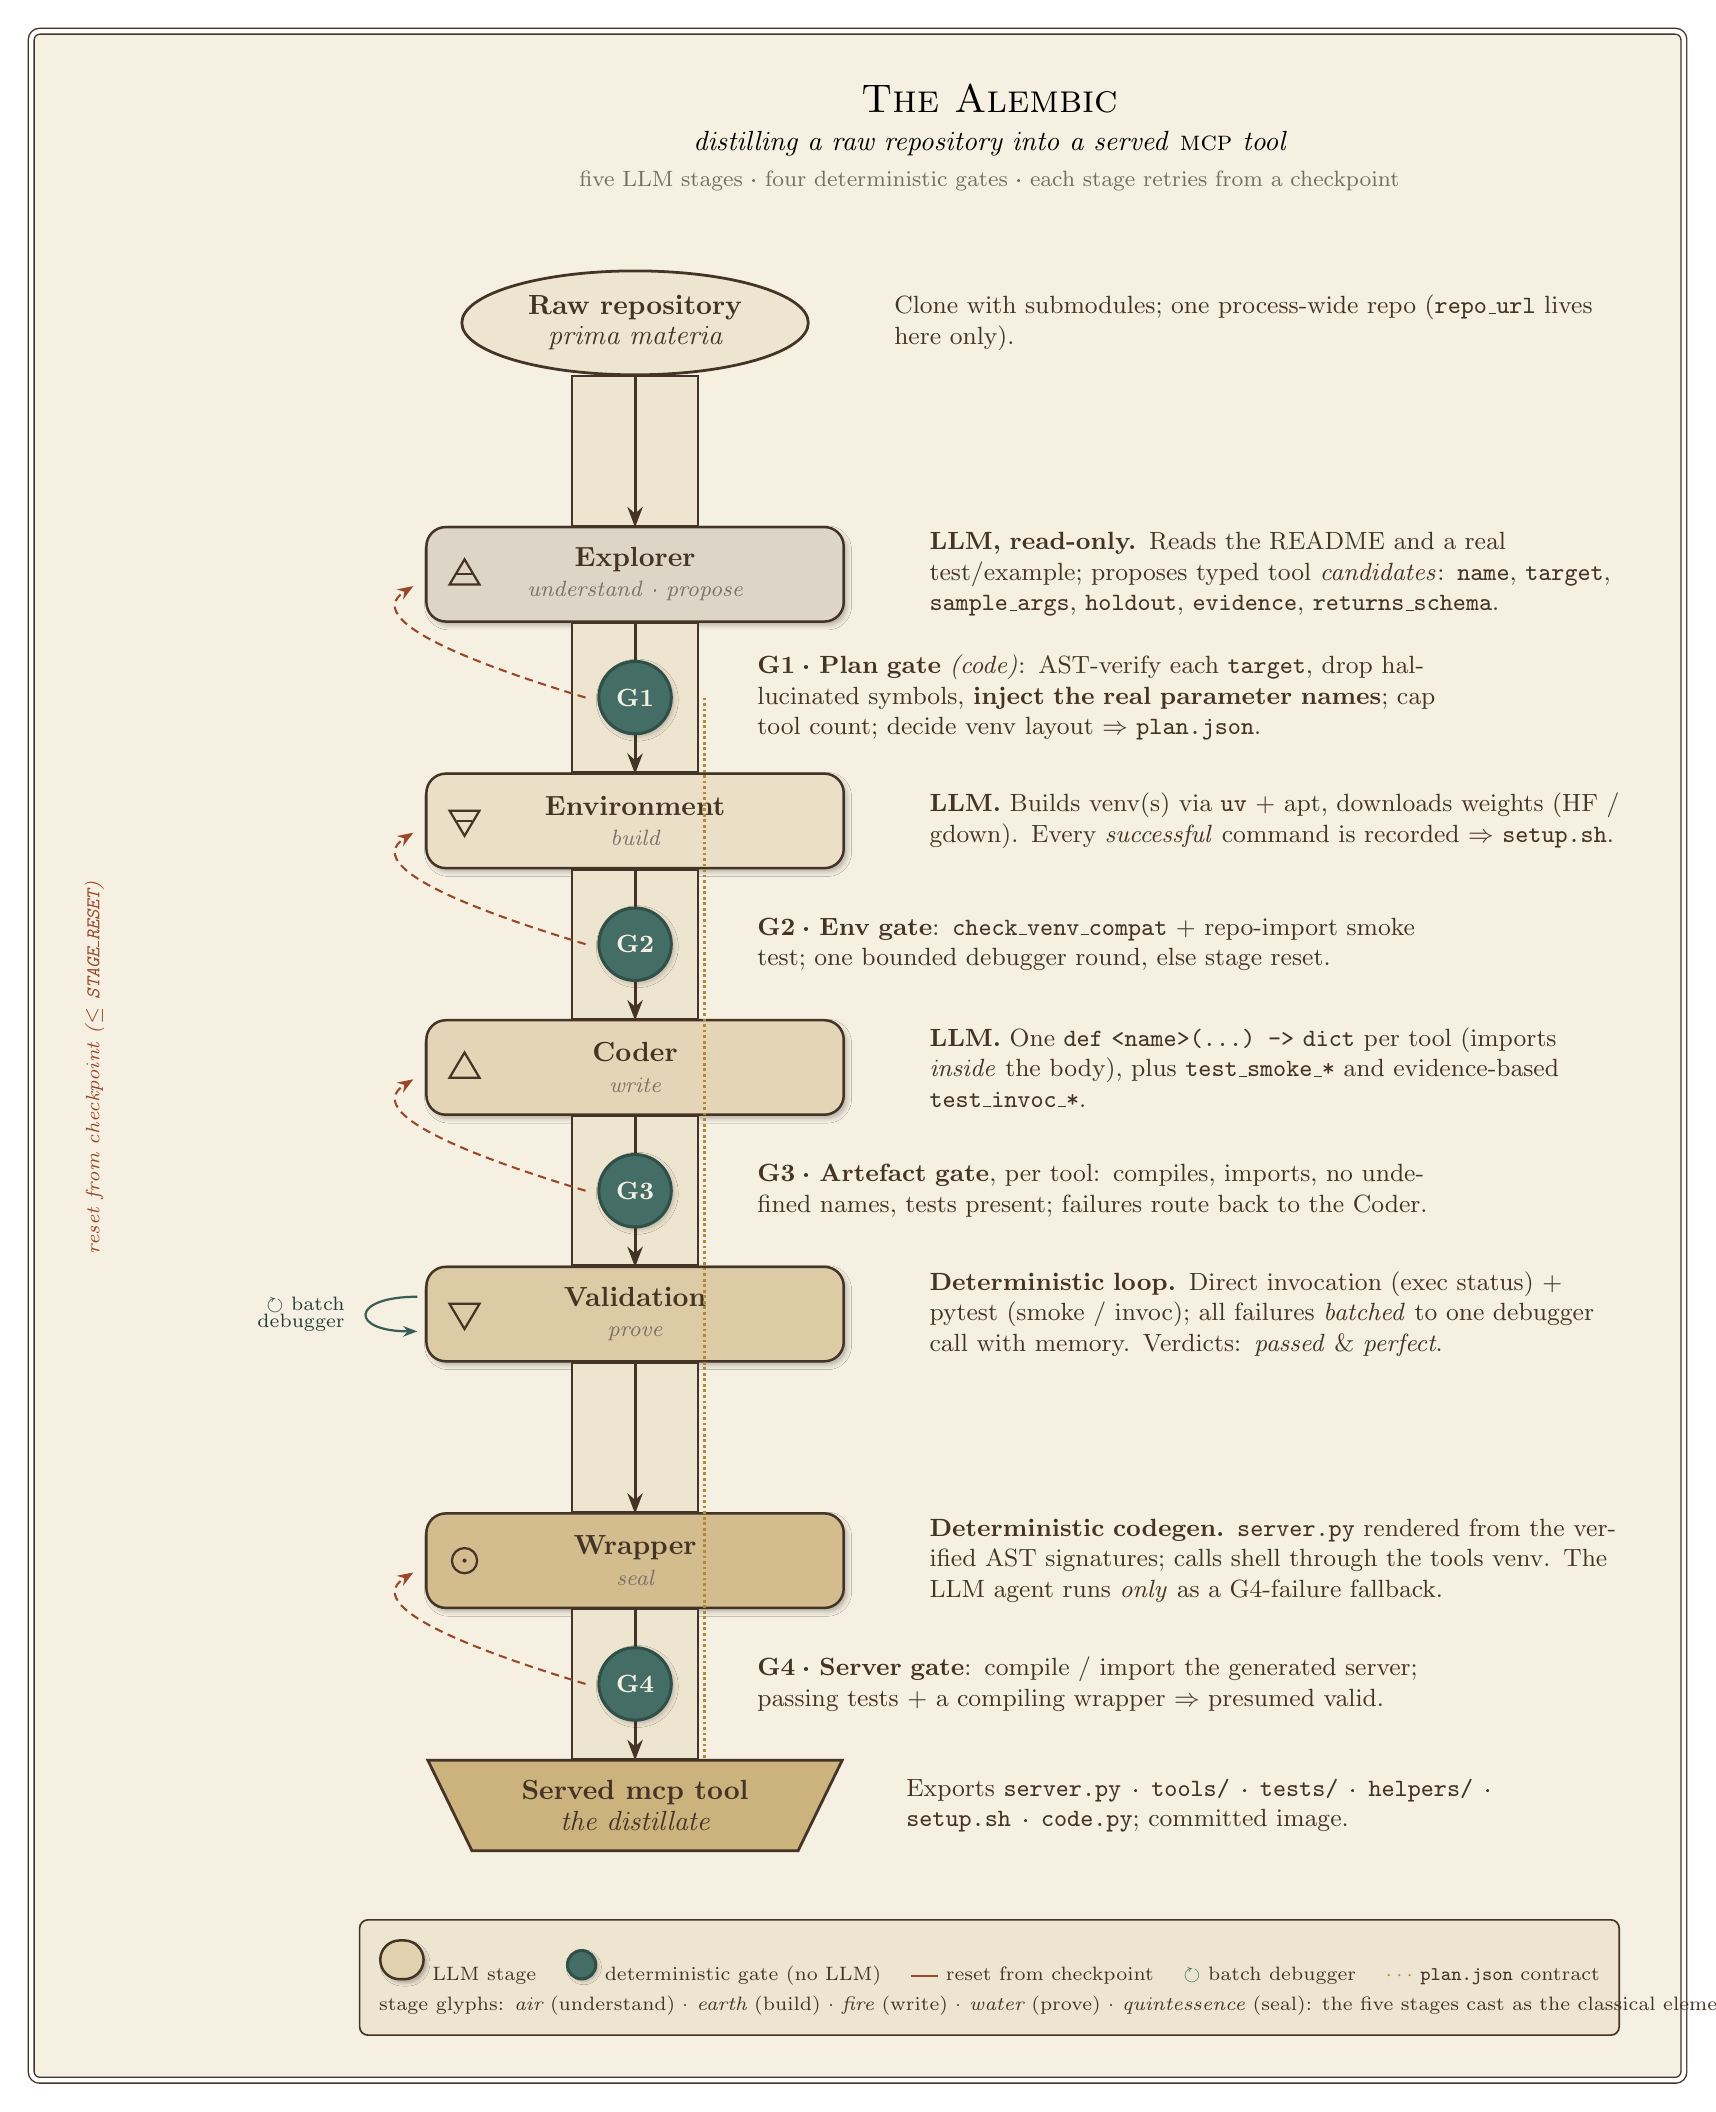
\begin{tikzpicture}[
   show background rectangle,
   background rectangle/.style={fill=parch, draw=ink, double, double distance=1.6pt,
       line width=0.5pt, rounded corners=3pt},
   inner frame sep=16pt,
   node distance=1.9cm and 0pt]

% =================== the column (top → bottom) =========================
\node[endcap, ellipse, fill=parchD, minimum width=4.4cm, minimum height=1.05cm]
   (inlet) {\bfseries Raw repository\\[-1pt]{\itshape prima materia}};

\node[vessel, fill=ink!14!parch, below=of inlet]      (explorer) {\role{Explorer}\\[-1pt]\subrole{understand \textperiodcentered\ propose}};
\node[vessel, fill=gold!16!parch, below=of explorer]  (environ)  {\role{Environment}\\[-1pt]\subrole{build}};
\node[vessel, fill=gold!26!parch, below=of environ]   (coder)    {\role{Coder}\\[-1pt]\subrole{write}};
\node[vessel, fill=gold!36!parch, below=of coder]     (validate) {\role{Validation}\\[-1pt]\subrole{prove}};
\node[vessel, fill=gold!50!parch, below=of validate]  (wrapper)  {\role{Wrapper}\\[-1pt]\subrole{seal}};

\node[endcap, below=of wrapper, trapezium, trapezium angle=64, shape border rotate=180,
   fill=gold!60!parch, minimum width=4.6cm, minimum height=1.15cm] (recv)
   {\bfseries Served \textsc{mcp} tool\\[-1pt]{\itshape the distillate}};

% =================== necks + downward flow =============================
\foreach \a/\b in {inlet/explorer, explorer/environ, environ/coder, coder/validate,
                   validate/wrapper, wrapper/recv}{
   \fill[neck] ([xshift=-0.8cm]\a.south) rectangle ([xshift=0.8cm]\b.north);
   \draw[flow] ($(\a.south)+(0,0.02)$) -- ($(\b.north)-(0,0.02)$);
}

% =================== gate valves (wax seals) on the necks ==============
\node[seal] (g1) at ($(explorer.south)!0.5!(environ.north)$) {G1};
\node[seal] (g2) at ($(environ.south)!0.5!(coder.north)$)    {G2};
\node[seal] (g3) at ($(coder.south)!0.5!(validate.north)$)   {G3};
\node[seal] (g4) at ($(wrapper.south)!0.5!(recv.north)$)     {G4};

% =================== element glyphs (inside each vessel, left) =========
\foreach \n in {explorer,environ,coder,validate,wrapper}{\coordinate (e-\n) at ([xshift=0.5cm]\n.west);}
% air (explorer): up-triangle + bar
\draw[ink,line width=0.8pt] ($(e-explorer)+(0,0.19)$)--($(e-explorer)+(-0.19,-0.13)$)--($(e-explorer)+(0.19,-0.13)$)--cycle;
\draw[ink,line width=0.8pt] ($(e-explorer)+(-0.1,0)$)--($(e-explorer)+(0.1,0)$);
% earth (environ): down-triangle + bar
\draw[ink,line width=0.8pt] ($(e-environ)+(0,-0.19)$)--($(e-environ)+(-0.19,0.13)$)--($(e-environ)+(0.19,0.13)$)--cycle;
\draw[ink,line width=0.8pt] ($(e-environ)+(-0.1,0)$)--($(e-environ)+(0.1,0)$);
% fire (coder): up-triangle
\draw[ink,line width=0.8pt] ($(e-coder)+(0,0.19)$)--($(e-coder)+(-0.19,-0.13)$)--($(e-coder)+(0.19,-0.13)$)--cycle;
% water (validate): down-triangle
\draw[ink,line width=0.8pt] ($(e-validate)+(0,-0.19)$)--($(e-validate)+(-0.19,0.13)$)--($(e-validate)+(0.19,0.13)$)--cycle;
% quintessence (wrapper): circle + dot
\draw[ink,line width=0.8pt] (e-wrapper) circle (0.16); \fill[ink] (e-wrapper) circle (0.026);

% =================== reset-from-checkpoint loops (left margin) =========
\foreach \g/\s in {g1/explorer, g2/environ, g3/coder, g4/wrapper}{
   \draw[reset] ([xshift=-0.15cm]\g.west) to[out=163,in=212,looseness=0.9]
        ([xshift=-0.15cm,yshift=-0.15cm]\s.west);
}
\node[font=\scriptsize\itshape, text=ember, rotate=90, align=center]
   at ([xshift=-4.2cm]coder.west) {reset from checkpoint ($\leq$ \texttt{STAGE\_RESET})};

% =================== validation batch-debugger self-loop (left) =======
\draw[verd!85!black, line width=0.8pt, -{Stealth[length=1.8mm]}]
   ([xshift=-0.1cm,yshift=0.22cm]validate.west) to[out=180,in=180,looseness=5]
   ([xshift=-0.1cm,yshift=-0.22cm]validate.west);
\node[font=\scriptsize, text=verd!55!black, anchor=east, align=right]
   at ([xshift=-0.9cm]validate.west) {$\circlearrowright$ batch\\[-2pt]debugger};

% =================== plan.json contract thread (right of column) ======
% gold conduit carrying the structured contract downstream (labelled in legend)
\draw[gold, line width=1pt, densely dotted] ([xshift=0.4cm]g1.east|-g1)
   -- ([xshift=0.4cm]g1.east|-recv.north);

% =================== captions (right of the column) ===================
\newcommand{\rcap}[2]{\node[descbox] at ([xshift=0.95cm]#1.east) {#2};}
\rcap{inlet}{Clone with submodules; one process-wide repo (\texttt{repo\_url} lives here only).}
\rcap{explorer}{\textbf{LLM, read-only.} Reads the README and a real test/example; proposes
   typed tool \emph{candidates}: \texttt{name}, \texttt{target}, \texttt{sample\_args},
   \texttt{holdout}, \texttt{evidence}, \texttt{returns\_schema}.}
\rcap{g1}{\textbf{G1 \textperiodcentered\ Plan gate} \emph{(code)}: AST-verify each \texttt{target},
   drop hallucinated symbols, \textbf{inject the real parameter names}; cap tool count;
   decide venv layout $\Rightarrow$ \texttt{plan.json}.}
\rcap{environ}{\textbf{LLM.} Builds venv(s) via \texttt{uv} $+$ apt, downloads weights (HF / gdown).
   Every \emph{successful} command is recorded $\Rightarrow$ \texttt{setup.sh}.}
\rcap{g2}{\textbf{G2 \textperiodcentered\ Env gate}: \texttt{check\_venv\_compat} $+$ repo-import smoke
   test; one bounded debugger round, else stage reset.}
\rcap{coder}{\textbf{LLM.} One \texttt{def <name>(...) -> dict} per tool (imports \emph{inside} the
   body), plus \texttt{test\_smoke\_*} and evidence-based \texttt{test\_invoc\_*}.}
\rcap{g3}{\textbf{G3 \textperiodcentered\ Artefact gate}, per tool: compiles, imports, no undefined
   names, tests present; failures route back to the Coder.}
\rcap{validate}{\textbf{Deterministic loop.} Direct invocation (exec status) $+$ pytest
   (smoke / invoc); all failures \emph{batched} to one debugger call with memory.
   Verdicts: \emph{passed} \& \emph{perfect}.}
\rcap{wrapper}{\textbf{Deterministic codegen.} \texttt{server.py} rendered from the verified AST
   signatures; calls shell through the tools venv. The LLM agent runs \emph{only} as a
   G4-failure fallback.}
\rcap{g4}{\textbf{G4 \textperiodcentered\ Server gate}: compile / import the generated server; passing
   tests $+$ a compiling wrapper $\Rightarrow$ presumed valid.}
\rcap{recv}{Exports \texttt{server.py \textperiodcentered\ tools/ \textperiodcentered\ tests/ \textperiodcentered\
   helpers/ \textperiodcentered\ setup.sh \textperiodcentered\ code.py}; committed image.}

% =================== title =============================================
\node[anchor=south, align=center] at (4.5,1.55)
  {{\scshape\Large The Alembic}\\[2pt]
   {\itshape distilling a raw repository into a served \textsc{mcp} tool}\\[1pt]
   {\footnotesize\color{ink!72} five LLM stages \textperiodcentered\ four deterministic gates \textperiodcentered\ each stage retries from a checkpoint}};

% =================== legend ============================================
\coordinate (legc) at (4.5,0);
\node[draw=ink, line width=0.6pt, rounded corners=3pt, fill=parchD, inner sep=7pt,
      anchor=north, align=left, font=\scriptsize, text=ink]
   at ($(legc|-recv.south)+(0,-0.85)$) {%
   \tikz\node[vessel, minimum width=0.55cm, minimum height=0.3cm, fill=gold!30!parch]{};\ LLM stage
   \hspace{8pt}\tikz\node[seal, minimum size=0.36cm]{};\ deterministic gate (no LLM)
   \hspace{8pt}{\color{ember}\rule[1.4pt]{10pt}{0.7pt}}\ reset from checkpoint
   \hspace{8pt}{\color{verd}$\circlearrowright$}\ batch debugger
   \hspace{8pt}{\color{gold}$\cdots$}\ \texttt{plan.json} contract\\[3pt]
   \makebox[0pt][l]{stage glyphs: {\itshape air} (understand) \textperiodcentered\ {\itshape earth} (build)
     \textperiodcentered\ {\itshape fire} (write) \textperiodcentered\ {\itshape water} (prove) \textperiodcentered\
     {\itshape quintessence} (seal): the five stages cast as the classical elements}};

\end{tikzpicture}
\end{document}
